\documentclass[12pt]{report}
\usepackage{titlesec}
\usepackage[utf8]{inputenc}
\usepackage[latvian]{babel}
\usepackage{enumitem}
\usepackage{fancyhdr}
\usepackage{gensymb} % grādu simbols
\usepackage{geometry}
\usepackage{graphicx}
\usepackage{hyperref}
\usepackage{array}
\usepackage{indentfirst}
\usepackage{multicol}
\usepackage{multirow}
\usepackage{ragged2e}
\usepackage{secdot}
\usepackage{tabularx}
\usepackage{tcolorbox}
\usepackage{tikz}
\usepackage{listings}
\usepackage{tocloft}
\usepackage{caption}
\usepackage{fmtcount}
\usepackage{ltablex}
\usepackage{chngcntr}
\usepackage{longtable}
\usepackage{ifthen}
\usepackage{needspace}
\usepackage[framemethod=TikZ]{mdframed}
% uncomment and comment the line above if compile time is too long for preview,
% but it won't compile the continuation overlay in the boxes correctly (should
% be commented for end compilation)
% \usepackage{mdframed}
\usetikzlibrary{positioning}

\hypersetup{
	colorlinks=true,
	linkcolor=black,
	urlcolor=black
}

\urlstyle{rm}

\renewcommand{\contentsname}{Saturs}

\titlespacing*{\section}{0pt}{2em}{2em}
\titlespacing*{\subsection}{0pt}{2em}{2em}
\titlespacing*{\subsubsection}{0pt}{2em}{2em}
\titlespacing*{\paragraph}{0pt}{2em}{2em}
\titlespacing*{\subparagraph}{0pt}{2em}{2em}



% Configure the chapter / paragraph numbering (it only works this way when I compile)
\renewcommand{\thechapter}{\arabic{chapter}.}
\renewcommand{\thesection}{\arabic{section}.}
\renewcommand{\thesubsection}{\thesection\arabic{subsection}.}
\renewcommand{\thesubsubsection}{\thesubsection\arabic{subsubsection}.}
\renewcommand{\theparagraph}{\thesubsubsection\arabic{paragraph}.}
\renewcommand{\thesubparagraph}{\theparagraph\arabic{subparagraph}.}


\titleformat{\section}{\large\bfseries\centering\vfill\eject\MakeUppercase}{\thesection}{1em}{} % section formatting
\titleformat{\subsection}{\bfseries}{\thesubsection}{1em}{} % subsection formatting
\titleformat{\subsubsection}{\bfseries}{\thesubsubsection}{1em}{} % subsubsection formatting
\titleformat{\paragraph}{\bfseries}{\theparagraph}{1em}{} % paragraph formatting
\titleformat{\subparagraph}{\bfseries}{\thesubparagraph}{0em}{} % subparagraph formatting


% Modify caption style
\DeclareCaptionFormat{format}{\textit{#1} \textbf{#3}}
\captionsetup{format=format}

\DeclareCaptionLabelFormat{image}{#2 att.}
\captionsetup[figure]{labelformat=image, labelsep=period}

\counterwithin{figure}{section} % Reset figure counter within each section
\renewcommand{\thefigure}{\thesection\arabic{figure}.} % Redefine figure numbering
\counterwithin{table}{section} % Reset table counter within each section
\renewcommand{\thetable}{\thesection\arabic{table}.} % Redefine table numbering

\captionsetup[table]{justification=raggedleft,singlelinecheck=off} % Align table caption text to the left
\captionsetup[figure]{justification=raggedright,singlelinecheck=off} % Align figure caption text to the right



\geometry{a4paper, left=30mm, right=20mm, top=20mm, bottom=20mm}

\pagestyle{fancy}
\fancyhead{}
\fancyfoot{}
\fancyfoot[C]{\thepage}
\renewcommand{\headrulewidth}{0pt}
\linespread{1.5}
\setlength{\parindent}{1cm}
\setlength{\parskip}{0pt}

\setcounter{secnumdepth}{5} % Numering for subsubsections
\setcounter{tocdepth}{3} % Add subsubsections in ToC


% ToC config
% TODO: section in uppercase
\renewcommand{\cftsecfont}{\MakeUppercase}
\renewcommand{\cfttoctitlefont}{\hfill\large\bfseries\MakeUppercase}
\renewcommand{\cftaftertoctitle}{\hfill}
\cftsetindents{section}{0.5cm}{0.5cm}
\cftsetindents{subsection}{1cm}{1cm}
\cftsetindents{subsubsection}{1.5cm}{1.5cm}
% \addto\captionslatvian{
% 	\renewcommand{\contentsname}{Satura rādītājs}
% }



\newcounter{rownum}
\renewcommand{\therownum}{\padzeroes[2]{\decimal{rownum}}}

\keepXColumns

% \newcommand{\moduleFunctionTable}[9]{
% 	\begin{tabularx}{\linewidth}{|X|}
% 		\caption{#1}\label{tab:#2}                                   \\ \hline
% 		\endfirsthead
%
% 		\hline \multicolumn{1}{r}{Turpinājums no iepriekšējās lapas} \\ \hline
% 		\endhead
%
% 		\hline \multicolumn{1}{r}{Turpinājums nākamajā lapā}         \\ \hline
% 		\endfoot
%
% 		\hline
% 		\endlastfoot
%
% 		\textbf{Funkcijas nosaukums}                                 \\ \hline
% 		#3                                                           \\ \hline
% 		\textbf{Funkcijas identifikators}                            \\ \hline
% 		#4                                                           \\ \hline
% 		\textbf{Ievads}                                              \\ \hline
% 		#5                                                           \\ \hline
% 		\textbf{Ievade}                                              \\ \hline
% 		#6                                                           \\ \hline
% 		\textbf{Apstrāde}                                            \\ \hline
% 		#7                                                           \\ \hline
% 		\textbf{Izvade}                                              \\ \hline
% 		#8                                                           \\ \hline
% 		\textbf{Paziņojumi}                                          \\ \hline
% 		#9                                                           \\ \hline
% 	\end{tabularx}
% }


\newcommand{\moduleFunctionTable}[9]{
	\paragraph{#1} \label{tab:#2}
	\textbf{Funkcijas nosaukums}: #3

	\textbf{Funkcijas identifikators}: #4

	\textbf{Ievads}: #5

	\textbf{Ievade}:

	#6

	\textbf{Apstrāde}: #7

	\textbf{Izvade}: #8

	\textbf{Paziņojumi}: #9
}




\begin{document}
\begin{titlepage}
    \thispagestyle{empty}
    \begin{center}
        \vspace*{2cm}
        \begin{large}\textbf{LATVIJAS UNIVERSITĀTE}

            \textbf{DATORIKAS FAKULTĀTE}

            \vfill
            \textbf{Mafia}
        \end{large}

        \vfill
        \textbf{Programminženierija}
    \end{center}
    \vspace{4cm}
    \begin{flushleft}
        \textbf{Alens Aleksandrs Čerņa}, ac22065

        \textbf{Ernests Gustavs Dane}, eg22086

        \textbf{Jorens Štekeļs} js21283

        \textbf{Kristiāns Francis Cagulis}, kc22015

        \textbf{Miķelis Kukainis}, mk22092
    \end{flushleft}
    \vspace{1cm}
    \begin{center}
        RĪGA 2023
    \end{center}
\end{titlepage}

\chapter*{Anotācija}
\setcounter{page}{2}
\lipsum[1-3]

\chapter*{Abstract}
\lipsum[1-3]

\pagebreak
\tableofcontents
\section*{Ievads}
\addcontentsline{toc}{section}{Ievads}
\subsection*{Nolūks}
Šī dokumenta mērķis ir raksturot tiešsaistes platformas ``MAFIJA'' programmatūras prasības.
Sistēma ir paredzēta individuāliem lietotājiem, kuru interesēs ir iesaistīties savstarpējā sociālā aktivitātē lomu spēles formātā.

\subsection*{Darbības sfēra}

Sistēma ``Mafija'' ir atvasināta no plaši pazīstamas sociālas lomu spēles, kas
balstās dedukcijā. Spēlē piedalās indivīdi - Spēlētāji, kas sadalīti vairākās
grupās un tajās ietvertās lomās. Lomu grupa ``Ciems'' lomas ``Iedzīvotājs''
ietvaros cenšas izdibināt kuri ir lomu grupas ``Mafija'' locekļi. Mafijas mērķis
ir radīt haosu ciema iedzīvotāju vidū un pakāpeniski izslēgt ciema iedzīvotājus
no spēles, izmantojot stratēģisku manipulāciju vai iedalītās lomas darbības.
Spēlētāji, kuri nav ietverti ne ``Ciems'', ne ``Mafija'' lomu grupā cenšas sasniegt
tiem iedalītās lomas mērķi. Tikai ``Mafijas'' locekļiem ir informācija par to,
kuri no spēlētāju loka pieder ``Mafija'' lomu grupai. Katram spēlētājam jāizmanto
individuāla ierīce, kas var pieslēgties tīmeklim, lai pieteiktos sistēmā,
pievienotos konkrētajai spēlei un piedalītos tajā.

Katra spēlētāja ierīcē spēles sesijas laikā tiek parādīta informācija par
iedalīto lomu un ar to saistītajām, pieejamajām darbībām, kuru nav paredzēts
vai atļauts rādīt citiem spēlētājiem. Sistēmas vizuālā saskarne ietver
informāciju par spēles aktuālo stāvokli, precīzāk, fāzi (diena / nakts), spēles
ilgumu, palikušo spēlētāju skaitu un citiem spēli raksturojošiem faktoriem.

Spēlētāja darbību klāsts ir atkarīgas no iedalītās lomas un aktuālā spēles
stāvokļa. Spēles organizatoram (maksas lietotājam) ir iespēja izveidot virtuālu
telpu un pielāgot tās iestatījumus, lai organizētu spēli vai mainītu to
konfigurāciju, kas ietver noteiktās lomas, kā arī mainīt un veidot jaunas
lomas.

Katram spēlētājam tiek nodrošināta sinhronizēta informācija par spēles tekošo
stāvokli un pieejamajām darbībām, tai skaitā, paziņojumi par spēles stāvokļa
izmaiņām.

Ārpus spēles sesijas, lietotājiem ir pieejams spēļu istabu saraksts, kas var
ietvert gan atvērtas, gan privātas virtuālās spēļu telpas, statistikas
pārskats, kurā pieejama statistika par jau izspēlētajām spēlēm, un lietotāja
profils, kurā var rediģēt lietotāju raksturojošo informāciju.

\subsection*{Saistība ar citiem dokumentiem}
PPS ir izstrādāta, ievērojot LVS 68:1996 ``Programmatūras prasību
specifikācijas ceļvedis`` un LVS 72:1996 ''Ieteicamā prakse programmatūras
projektējuma aprakstīšanai” standarta prasības.

\subsection*{Pārskats}

Dokumenta ievads satur tā nolūku, izstrādājamās programmatūras skaidrojumu,
vispārīgu programmatūras mērķi un funkciju klāstu, saistību ar citiem
dokumentiem, kuru prasības tika izmantotas dokumenta izstrādāšanas gaitā, kā
arīpārskatu par dokumenta daļu saturu ar dokumenta struktūras skaidrojumu.

Pirmajā nodaļa tiek aprakstīti faktori, kas var ietekmēt produktu un tā
prasības. Nodaļā tiek pamatota programmatūras izstrādes motivācija un nolūks,
aprakstītas produkta vieta citu sistēmu perspektīvā, galvenās augsta līmeņa
darījumprasības, sistēmas lietotāju grupu lomas un mērķi, kā arī tiek
uzskaitīti faktori, kas var ierobežot vai ietekmēt programmatūras prasību
specifikāciju.

Otrajā nodaļā tiek norādītas konkrētas prasības, kas satur visu nepieciešamo
programmatūras projektējuma veidošanai. Tā ietver: datu bāzes konceptuālo
modeli, funkcionālās prasības, kas apraksta sistēmas funkciju sadalījumu pa
moduļiem, arējās saskarnes prasības un sistēmas vispārējās prasības.

Trešajā nodaļā tiek aprakstīts projektējums, kas ietver sistēmas sastāvdaļu
aprakstu. Nodaļa satur datu bāzes projektējumu, tās fizisko modeli un daļēju
funkciju un lietotāju saskarņu projektējumu. 


\section*{Apzīmējumu saraksts}
\addcontentsline{toc}{section}{Apzīmējumu saraksts}
MAFIJA - tiešsaistes lomu spēles platforma;

PPS - programmatūras prasību specifikācija;

ER modelis - entitāšu saišu modelis (angl. entity relationship model);

DPD - datu plūsmas diagramma;

LBPK - Uz lomu bāzēta piekļuves kontole;

Maksas siena - maksājums par lietotāju pieeju daļai no sistēmas piedāvātās funkcionalitātes;

Spēlētājs - lietotāja ieraksts vienas virtuālās istabas kontekstā.

\section{Vispārējais apraksts}
\subsection{Esošā stāvokļa apraksts}
Tirgū pastāv vairākas sistēmas un citi programmatūras formāti, piemēram,
lietotnes, kas piedāvā dažādas lomu spēļu variācijas, to skaitā, ``Warewolf
online'', ``Town of Salem'', ``Mafia.gg'', ``BeyondMafia'', ``Mafia: The Game''
un daudzi citi. Esošiem risinājumiem ir vairākas problēmas: maksas piekļuve,
pārmērīgs iespēju skaits, kas ir pieejamas tikai par maksu, spēle ir pieejama
tikai uz mobilā viedtālruņa. “Mafija” īstenos svarīgākās no esošo spēļu
iespējām un pievienos jaunas iespējas, kas papildinās un uzlabos lietotāju
pieredzi, kā arī samazinās maksas funkciju īpatsvaru.

\subsection{Pasūtītājs}
Sistēma nav izstrādāta pēc konkrēta pasūtītāja pieprasījuma, tā ir raksturota un projektēta ar iespēju realizēt pēc studentu grupas iniciatīvas programminženierijas kursa ietvaros.

\subsection{Produkta perspektīva}
Sistēmā tiek integrēti vai izmantoti citu uzņēmumu un izstrādātāju piedāvāti
pakalpojumi. Produkta realizācijā ir paredzēts izmantot maksājumu apstrādāšanas
pakalpojumus, kamēr tie atbilst sistēmas pieprasītajai funkcionalitātei un
piedāvā optimālākos, kā arī drošākos un efektīvākos risinājumus tirgū.

Maksājumu apstrādātājs realizēs lietotāju maksas pakalpojumu iegādi konkrētu
papildus funkciju iegūšanai uz noteiktu laiku. Abonementa detaļas tiek glabātas
sistēmā. Tiks izmantota pakalpojumu sniedzēja nodrošināta maksājumu apstrāde
ārpus ``MAFIJA'' sistēmas, glabājot minimālu informāciju, tas ir, klienta
identifikatoru.

\subsection{Darījumprasības}
Sistēmā ``MAFIJA'' tiks  realizētas sekojošās darījumprasības:
\begin{enumerate}
	\item Lietotāju reģistrācija, autentifikācija;
	\item Lietotāju un to privilēģiju pārvalde;
	\item Lietotāju konta apstiprināšana, izmantojot e-pastu;
	\item Lietotāju profilu personalizācija un kontu rediģešana;
	\item Lietotāju stāvokļa virtuālajās telpās uzturēšana un izmaiņa;
	\item Lietotāju informēšana, izmantojot paziņojumu sistēmu;
	\item Sinhronizēta spēles stāvokļa atjaunināšana;
	\item Spēles uzstādījumu un lomu klāsta publiska veidošana, rediģēšana un dzēšana;
	\item Publisko un privāto virtuālo spēles istabu pārvalde;
	\item Spēles automātiska vadība;
	\item Kopēja un ierobežotu grupu (lomu atkarīga) tērzēšana;
	\item Privilēģiju izmaiņa, izmantojot bezpersonisku maksājumu sistēmu;
	\item Lietotāju moderēšana;
\end{enumerate}

\subsection{Sistēmas lietotāji}

Neautentificēts lietotājs (viesis), i.e., viesis ir jebkurš lietotājs, kas nav
pieteicies vai reģistrējies sistēmā. Šiem lietotājiem ir pieejamas funkcijas,
lai reģistrētos vai pieteiktos sistēmā;

Kad lietotājs ir pieteicies un ir autentificēts, tam ir pieejamas reģistrēta
lietotāja grupas privilēģijas, precīzāk, darbības saistītas ar spēli, profilu
un konta pārvaldi. Tā būs vislielākā grupa pēc lietotāju skaita. Maksas
lietotājiem, precīzāk, reģistrētiem lietotājiem, kuriem piesaistīts aktīvs
abonements, tiek piešķirtas papildus funkcijas - izveidot jaunas virtuālās
istabas, izvēlēties spēles konfigurāciju savās istabās un citas. Maksas
lietotāja grupa ir atvasināta no reģistrēta lietotāja grupas.

Administratoru uzdevumi ietver istabu uzturēšanu un  lietotāju moderēšanu ar
darbībām, kā bloķēšana, spēles istabas un lietotāju stāvokļa izmainīšana, konta
informācijas izmaiņa, lomu uzstādījumu un spēles konfigurācijas rediģēšana.
Lietotājs ``Sistēma'' izpilda noteiktas, ar spēles gaitu saistītas darbības, kas
notiek automātiski un kas nav tiešā veidā citu lietotāju grupu kompetencēs.

Ar lietotājiem saistītās datu plūsmas ir attēlotas sistēmas nultā līmeņa DPD (skat. \ref{fig:dpd-0} att.).


\begin{figure}[htbp]
	\centering
	\includegraphics[width=\linewidth]{./src/img/0tāLīmeņaDPD.png}
	\caption{0. līmeņa DPD}
	\label{fig:dpd-0}
\end{figure}

\subsection{Vispārējie ierobežojumi}
\begin{enumerate}

\begin{enumerate}
    \item Drošības un aizsardzības apsvērumi:
        \begin{enumerate}
            \item Lietotāju paroles tiek šifrētas pirms glabāšanas, izmantojot SHA-2 algoritmu;
            \item Tiek izmantota trešās puses autentifikācijas integrācija.
        \end{enumerate}
    \item Regulējošās politikas apsvērumi:
        \begin{enumerate}
            \item Tiek pieprasīta lietotāju atļauja realizēt analītisku datu ievākšanu, izmantojot sīkdatnes..
        \end{enumerate}
    \item Izstrādes vides, tehnoloģijas un tīmekļa ierobežojumi:
        \begin{enumerate}
            \item Programmēšanas valodas, to tehniskie ierobežojumi;
            \item Responsivitāte;
            \item Sistēmas saskarne ir tīmekļa vietne;
            \item Sistēmas ietvaros mitināta vietne ir kopīga neatkarīgi no ierīces (netiek izmantots apakšdomēns mobilo tālruņu lietotājiem).
        \end{enumerate}
\end{enumerate}

\subsection{Pieņēmumi un atkarības}
\begin{itemize}
	\item Platformu veidojošās datnes, datu bāzes, kontrolieri tiks mitināti pie viena mitināšanas pakalpojuma sniedzēja.
	\item Ierīce atbalsta un ļauj pilnā sistēmas funkcionalitātē pieslēgties sistēmai. Lietotāja ierīce ir sasniegusi minimālo vajadzības slieksni, lai izmantotu produktu, bez problēmām.
	\item Tiek pieņemts, ka lietotāja ierīcei ir stabils interneta savienojums. Bez stabila interneta savienojuma ir iespējami traucējumi lietotnes izmantošanā.
	\item Sistēmā būs integrēti maksājumu ārpakalpojumi. Sistēmā būs iespēja iegūt maksas pakalpojumus.
	\item Sistēma tiek veidota kā interneta lietotne, tāpēc ierobežojumi galvenokārt ir saistīti ar pārlūkprogrammu savietojamību. Tiek pieņemts, ka sistēmas lietotāji to lietos, izmantojot pārlūkprogrammas, kas atbalsta funkcionālas prasības, kas ir nepieciešamas, lai īstenotu korektu sistēmas darbību.
\end{itemize}


\section{Programmatūras prasību specifikācija}
\subsection{Konceptuālais datu bāzes apraksts}
Konceptuālajā modelī redzamās entītātes no konceptuālā ER modeļa (\ref{fig:conceptual-model} attēls):
\begin{itemize}
	\item Lietotājs - reģistrēts lietotājs, kas pieder noteiktai grupai;
	\item Attēls - datnes metadati un tās adrese, kas ir saistīta ar lietotāju vai spēles lomu;
	\item Maksas abonements - lietotāju maksas abonementa dati.
	\item Abonementa cena - cena par abonementu, kas darbojas noteiktā laika periodā.
	\item Spēles uzstādījums - vairāku spēles lomu kopa, kas ir izveidojamas arī publiski (maksas spēlētājiem)
	\item Spēles loma - spēlē izmantojamās lomas apraksts, katrai lomai obligāti piemīt trūkumi un darbības.
	      Tā var tikt izveidota publiski (analoģiski spēles uzstādījumiem);
	\item Lomas darbība - vienai vai vairākām spēles lomas piemītošās spēles darbības apraksts un spēlei specifiskie atribūti(/-s);
	\item Lomas trūkums - vienai vai vairākām spēles lomas piemītošā trūkuma apraksts;
	\item Spēlētājs - vienai virtuālai spēles istabai piederošais spēlētājs.
	      Tam piemīt viena spēles loma un var būt vairākas spēles gaitā veiktās
	      lomai atbilstošās darbības;
	\item Īsziņa - virtuālās istabas tērzēšanā izveidotā īsziņa, kas tiek saistīta ar vienu spēlētāju un var atbildēt uz citu īsziņu izveides laikā;
	\item Spēles notikums - spēles fāzes maiņa, spēlētāju izslēgšana, piemēram, izbalsošana vai slepkavība, un citi.
	\item Spēles virtuāla istaba - vienas gaidāmas, tekošās vai pagātnē notikušas spēles, kam piemīt spēlētāji, spēles uzstādījumi, spēles notikumi, izveidotājs (lietotājs maskas lietotāja grupā);
\end{itemize}

\begin{figure}[htbp]
	\centering
	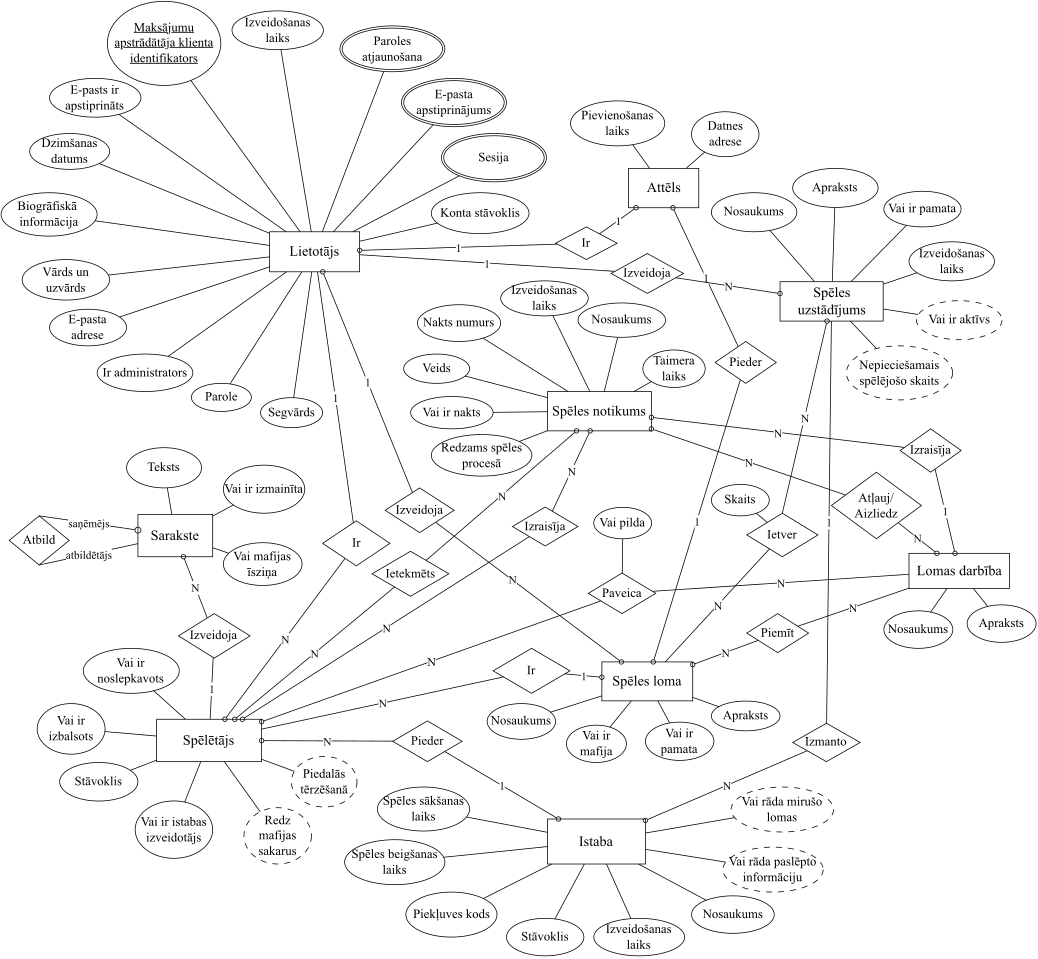
\includegraphics[width=\linewidth]{./src/img/KonceptualaisERModelis.png}
	\caption{Datu bāzes konceptuālais ER modelis}
	\label{fig:conceptual-model}
\end{figure}

\subsection{Funkcionālās prasības}
\subsubsection{Vispārīgi paziņojumi}

\begin{tabularx}{\linewidth}{|p{2.5cm}|X|p{2.7cm}|X|}
	\caption{Vispārīgi paziņojumi} \label{tab:general_notices}                                                                                                                                                                                                             \\
	\hline
	\textbf{Paziņojumu grupa}                                & \textbf{Paziņojums}                                                                                                & \textbf{Identifikators}           & \textbf{Raksturojums}                              \\
	\hline
	\endfirsthead

	\multicolumn{4}{c}%
	{{\thetable{} \tablename: turpinājums no iepriekšējās lapas}}                                                                                                                                                                                                          \\
	\hline
	\textbf{Paziņojumu grupa}                                & \textbf{Paziņojums}                                                                                                & \textbf{Identifikators}           & \textbf{Raksturojums}                              \\
	\hline
	\endhead

	\hline \multicolumn{4}{|r|}{{Turpinājums nākamajā lapā}}                                                                                                                                                                                                               \\ \hline
	\endfoot

	\hline
	\endlastfoot

	% Table data here
	\setcounter{rownum}{0}
	\multirow{3}{2.5cm}{Vispārīgi kļūdu paziņojumi}          & ``Iesniegtā datne pārsniedz maksimālo pieļaujamo datnes lielumu. Lūdzu, mēģiniet vēlreiz ar mazāka izmēra datni!'' & \stepcounter{rownum}VKP\therownum & Iesniegtā datne pārsniedz maksimālo datnes izmēru. \\ \cline{2-4}
	                                                         & ``Jūsu pieprasījums spēļu sistēmai nav korekts. Lūdzu, mēģiniet vēlreiz!''                                         & \stepcounter{rownum}VKP\therownum & \dots                                              \\ \cline{2-4}
	                                                         & ``Ir notikusi sistēmas iekšējā ķļūme. Lūdzu, mēģiniet vēlreiz!''                                                   & \stepcounter{rownum}VKP\therownum & \dots                                              \\ \hline
	\setcounter{rownum}{0}
	\multirow{5}{2.5cm}{Vispārīgi apstiprinājumu paziņojumi} & ``[Entitātes nosaukums] ir veiksmīgi izveidota(/-s)!''                                                             & \stepcounter{rownum}VAP\therownum & Lietotājs ir veiksmīgi izveidojis entitāti.        \\ \cline{2-4}
	                                                         & ``[Entitātes nosaukums] ir veiksmīgi rediģēta(/-s)!''                                                              & \stepcounter{rownum}VAP\therownum & Lietotājs ir veiksmīgi rediģējis entitāti.         \\ \cline{2-4}
	                                                         & ``[Entitātes nosaukums] ir veiksmīgi rediģēta(/-s)!''                                                              & \stepcounter{rownum}VAP\therownum & Lietotājs ir veiksmīgi rediģējis entitāti.         \\ \cline{2-4}
	                                                         & ``[Entitātes nosaukums] ir veiksmīgi rediģēta(/-s)!''                                                              & \stepcounter{rownum}VAP\therownum & Lietotājs ir veiksmīgi rediģējis entitāti.         \\ \cline{2-4}
	                                                         & ``[Entitātes nosaukums] ir veiksmīgi rediģēta(/-s)!''                                                              & \stepcounter{rownum}VAP\therownum & Lietotājs ir veiksmīgi rediģējis entitāti.         \\ \hline
	\setcounter{rownum}{0}
	\parbox{2.5cm}{Vispārīgi informācijas paziņojumi}        &                                                                                                                    & \stepcounter{rownum}VIP\therownum &                                                    \\ \hline
	\setcounter{rownum}{0}
	\parbox{2.5cm}{Vispārīgi spēles paziņojumi??}            &                                                                                                                    & \stepcounter{rownum}VSP\therownum &                                                    \\ \hline
	% ... continue for each row
\end{tabularx}

\subsubsection{Citas apakšnodaļas ar vispārīgu lietu aprakstu}
\subsubsection{Funkciju sadalījums moduļos}
Funkciju sadalījums moduļos ir aprakstīts tabulā (\ref{tab:function-modules} tab.).
Katrs maksas lietotājs un administrators ir uzskatāms par reģistrētu lietotāju.
Administratora privilēģijas ir atvasinātas no maksas lietotāja privilēģijas.
Sistēmas lietotājs nav ierobežots.
Maksas lietotājs un administrators tiek norādīts pie lietotāja grupas tikai tad, ja, funkcijas rezultāts atšķiras no rezultāta, kuru atgrieztu reģistrētam lietotājam.
Tiek pieņemts, ka lietotāja autentifikācija ir izpildīta, izmantojot funkcijas, kur apstrāde ir neatkarīga no lietotāju grupas.

2.līmeņa DPD parāda izvērstāku 1. līmeņa (jeb konteksta) DPD ar sistēmas sadalījumu pa moduļiem.
Pārskatāmības dēļ DPD tika sadalīta divās daļās (skat \ref{fig:dpd-1.1} att. un \ref{fig:dpd-1.2} att.).


\begin{figure}[htbp]
	\centering
	\includegraphics[width=\linewidth]{./src/img/1LīmeņaDPDSpēlesDatubāze.png}
	\caption{1. līmeņa DPD (1)}
	\label{fig:dpd-1.1}
\end{figure}

\begin{figure}[htbp]
	\centering
	\includegraphics[width=\linewidth]{./src/img/1LīmeņaDPDLietotājuDatubāze.png}
	\caption{1. līmeņa DPD (2)}
	\label{fig:dpd-1.2}
\end{figure}
\eject


\begin{tabularx}{\linewidth}{|p{2.1cm}|X|p{2.7cm}|X|}
	\caption{Funkciju sadalījums pa moduļiem} \label{tab:function-modules}                                                                                                                                                                                    \\ \hline

	\hline
	\textbf{Modulis}                                           & \textbf{Funkcija}                                      & \textbf{Identifikators}                                                             & \textbf{Lietotāja grupa}                      \\ \hline
	\endfirsthead

	\hline \multicolumn{4}{r}{Turpinājums no iepriekšējās lapas}                                                                                                                                                                                              \\ \hline
	\textbf{Modulis}                                           & \textbf{Funkcija}                                      & \textbf{Identifikators}                                                             & \textbf{Lietotāja grupa}                      \\ \hline
	\endhead

	\hline \multicolumn{4}{r}{Turpinājums nākamajā lapā}                                                                                                                                                                                                      \\ \hline
	\endfoot

	\hline
	\endlastfoot


	% Table data here
	\setcounter{rownum}{0}
	\multirow{1}{2.1cm}{Reģistrācijas un pieteikšanās modulis} & Lietotāja reģistrācija                                 & \hyperref[tab:mod-func-auth-reg]{\stepcounter{rownum}AMF\therownum}                 & Nereģistrēts lietotājs                        \\ \cline{2-4}
	                                                           & Apstiprinājuma ziņas atkārtotās izsūtīšanas pieteikums & \hyperref[tab:mod-func-auth-app]{\stepcounter{rownum}AMF\therownum}                 & Nereģistrēts lietotājs, Reģistrēts lietotājs  \\ \cline{2-4}
	                                                           & Paroles atjaunošanas pieteikums                        & \hyperref[tab:mod-func-auth-pass-restore-app]{\stepcounter{rownum}AMF\therownum}    & Reģistrēts lietotājs                          \\ \cline{2-4}
	                                                           & Paroles atjaunošana                                    & \hyperref[tab:mod-func-auth-pass-restore]{\stepcounter{rownum}AMF\therownum}        & Reģistrēts lietotājs                          \\ \cline{2-4}
	                                                           & Lietotāja pieteikšanās                                 & \hyperref[tab:mod-func-auth-login]{\stepcounter{rownum}AMF\therownum}               & Reģistrēts lietotājs                          \\ \cline{2-4}
	                                                           & Lietotāja atteikšanās                                  & \hyperref[tab:mod-func-auth-logout]{\stepcounter{rownum}AMF\therownum}              & Reģistrēts lietotājs                          \\ \cline{2-4}
	                                                           & Lietotāja konta apstiprināšana                         & \hyperref[tab:mod-func-auth-email-confirm]{\stepcounter{rownum}AMF\therownum}       & Reģistrēts lietotājs                          \\ \hline

	\setcounter{rownum}{0}
	\multirow{1}{2.1cm}{Lietotāju kontu modulis}               & Lietotāju profilu pārskats                             & \hyperref[tab:mod-func-user-profiles]{\stepcounter{rownum}LAM\therownum}            & Reģistrēts lietotājs, Administrators          \\ \cline{2-4}
	                                                           & Lietotāja konta detaļas                                & \hyperref[tab:mod-func-user-profile-data]{\stepcounter{rownum}LAM\therownum}        & Reģistrēts lietotājs, Administrators          \\ \cline{2-4}
	                                                           & Lietotāja konta bloķēšana                              & \hyperref[tab:mod-func-user-block]{\stepcounter{rownum}LAM\therownum}               & Administrators                                \\ \cline{2-4}
	                                                           & Lietotāja konta rediģēšana                             & \hyperref[tab:mod-func-user-edit]{\stepcounter{rownum}LAM\therownum}                & Reģistrēts lietotājs, Administrators          \\ \cline{2-4}
	                                                           & Lietotāja konta dzēšāna                                & \hyperref[tab:mod-func-user-delete]{\stepcounter{rownum}LAM\therownum}              & Reģistrēts lietotājs, Administrators          \\ \hline
	\setcounter{rownum}{0}
	\multirow{1}{2.1cm}{Maksas abonamentu modulis}             & Abonementa pieteikums                                  & \hyperref[tab:mod-func-premium-app]{\stepcounter{rownum}MAMF\therownum}             & Reģistrēts lietotājs                          \\ \cline{2-4}
	                                                           & Abonementu pārskats                                    & \hyperref[tab:mod-func-premium-overview]{\stepcounter{rownum}MAMF\therownum}        & Reģistrēts lietotājs, Maksas lietotājs        \\ \cline{2-4}
	                                                           & Abonementa atcelšana                                   & \hyperref[tab:mod-func-premium-cancel]{\stepcounter{rownum}MAMF\therownum}          & Maksas lietotājs, Administrators              \\ \hline

	\setcounter{rownum}{0}
	\multirow{1}{2.1cm}{Cenu modulis}                          & Cenas pievienošana                                     & \hyperref[tab:mod-func-price-add]{\stepcounter{rownum}CMF\therownum}                & Administrators                                \\ \cline{2-4}
	                                                           & Cenas rediģēšana                                       & \hyperref[tab:mod-func-price-edit]{\stepcounter{rownum}CMF\therownum}               & Administrators                                \\ \cline{2-4}
	                                                           & Cenu pārskats                                          & \hyperref[tab:mod-func-price-overview]{\stepcounter{rownum}CMF\therownum}           & Administrators                                \\ \hline
	\setcounter{rownum}{0}
	\multirow{1}{2.1cm}{Tērzēšanas modulis}                    & Jaunas īsziņas izveidošana                             & \hyperref[tab:mod-func-chat-create]{\stepcounter{rownum}TMF\therownum}              & Reģistrēts lietotājs                          \\ \cline{2-4}
	                                                           & Īsziņas dzēšana                                        & \hyperref[tab:mod-func-chat-delete]{\stepcounter{rownum}TMF\therownum}              & Reģistrēts lietotājs                          \\ \cline{2-4}
	                                                           & Īsziņu pārskats                                        & \hyperref[tab:mod-func-chat-overview]{\stepcounter{rownum}TMF\therownum}            & Reģistrēts lietotājs                          \\ \cline{2-4}
	                                                           & Īsziņu rediģēšana                                      & \hyperref[tab:mod-func-chat-edit]{\stepcounter{rownum}TMF\therownum}                & Reģistrēts lietotājs                          \\ \hline
	\setcounter{rownum}{0}
	\multirow{1}{2.1cm}{Spēles istabas modulis}                & Pieejamo pieslēgšanās spēles istabu pārskats           & \hyperref[tab:mod-func-room-overview]{\stepcounter{rownum}SIMF\therownum}           & Reģistrēts lietotājs                          \\ \cline{2-4}
	                                                           & Pieslēgšanās spēles istabai                            & \hyperref[tab:mod-func-room-connect]{\stepcounter{rownum}SIMF\therownum}            & Reģistrēts lietotājs                          \\ \cline{2-4}
	                                                           & Atslēgšanās no spēles istabas pieteikums               & \hyperref[tab:mod-func-room-disconnect]{\stepcounter{rownum}SIMF\therownum}         & Reģistrēts lietotājs                          \\ \cline{2-4}
	                                                           & Jaunas spēles istabas izveide                          & \hyperref[tab:mod-func-room-create]{\stepcounter{rownum}SIMF\therownum}             & Maksas lietotājs, Administrators              \\ \cline{2-4}
	                                                           & Spēles sākuma pieteikums                               & \hyperref[tab:mod-func-room-app]{\stepcounter{rownum}SIMF\therownum}                & Maksas lietotājs                              \\ \cline{2-4}
	                                                           & Spēlētāja izslēgšana                                   & \hyperref[tab:mod-func-room-kill]{\stepcounter{rownum}SIMF\therownum}               & Administrators                                \\ \cline{2-4}
	                                                           & Spēlētāju pārskata iegūšana                            & \hyperref[tab:mod-func-room-player-overview]{\stepcounter{rownum}SIMF\therownum}    & Sistēma, Reģistrēts lietotājs, Administrators \\ \hline
	\setcounter{rownum}{0}
	\multirow{1}{2.1cm}{Spēles gaitas modulis}                 & Spēles darbības veikšana                               & \hyperref[tab:mod-func-progress-action]{\stepcounter{rownum}SGMF\therownum}         & Reģistrēts lietotājs                          \\ \cline{2-4}
	                                                           & Spēles notikuma izveidošana                            & \hyperref[tab:mod-func-progress-create]{\stepcounter{rownum}SGMF\therownum}         & Sistēma                                       \\ \cline{2-4}
	                                                           & Spēles notikumu pārskats                               & \hyperref[tab:mod-func-progress-overview]{\stepcounter{rownum}SGMF\therownum}       & Sistēma, Reģistrēts lietotājs                 \\ \cline{2-4}
	                                                           & Spēles stāvokļa detaļas                                & \hyperref[tab:mod-func-progress-state-overview]{\stepcounter{rownum}SGMF\therownum} & Sistēma, Reģistrēts lietotājs                 \\ \hline
	\setcounter{rownum}{0}
	\multirow{1}{2.1cm}{Spēles lomu uzstādījumu modulis}       & Lomas detaļu detaļas                                   & \hyperref[tab:mod-func-role-details]{\stepcounter{rownum}SLMF\therownum}            & Reģistrēts lietotājs                          \\ \cline{2-4}
	                                                           & Lomu pārskats                                          & \hyperref[tab:mod-func-role-overview]{\stepcounter{rownum}SLMF\therownum}           & Reģistrēts lietotājs                          \\ \cline{2-4}
	                                                           & Lomas darbību pārskats                                 & \hyperref[tab:mod-func-role-action-overview]{\stepcounter{rownum}SLMF\therownum}    & Reģistrēts lietotājs                          \\ \cline{2-4}
	                                                           & Jaunas lomas izveidošana                               & \hyperref[tab:mod-func-role-create]{\stepcounter{rownum}SLMF\therownum}             & Maksas lietotājs, Administrators              \\ \cline{2-4}
	                                                           & Lomas rediģēšana                                       & \hyperref[tab:mod-func-role-edit]{\stepcounter{rownum}SLMF\therownum}               & Maksas lietotājs, Administrators              \\ \cline{2-4}
	                                                           & Lomas dzēšana                                          & \hyperref[tab:mod-func-role-delete]{\stepcounter{rownum}SLMF\therownum}             & Maksas lietotājs, Administrators              \\ \hline
	\setcounter{rownum}{0}
	\multirow{1}{2.1cm}{Spēles uzstādījumu modulis}            & Spēles uzstādījumu pārskats                            & \hyperref[tab:mod-func-setup-overview]{\stepcounter{rownum}SUMF\therownum}          & Reģistrēts lietotājs                          \\ \cline{2-4}
	                                                           & Spēles uzstādījumu lomu pārskats                       & \hyperref[tab:mod-func-setup-role-overview]{\stepcounter{rownum}SUMF\therownum}     & Reģistrēts lietotājs, Sistēma                 \\ \cline{2-4}
	                                                           & Jaunas spēles uzstādījuma izveidošana                  & \hyperref[tab:mod-func-setup-new]{\stepcounter{rownum}SUMF\therownum}               & Maksas lietotājs, Administrators              \\ \cline{2-4}
	                                                           & Spēles uzstādījuma rediģēšana                          & \hyperref[tab:mod-func-setup-edit]{\stepcounter{rownum}SUMF\therownum}              & Maksas lietotājs, Administrators              \\ \cline{2-4}
	                                                           & Spēles uzstādījuma dzēšana                             & \hyperref[tab:mod-func-setup-delete]{\stepcounter{rownum}SUMF\therownum}            & Maksas lietotājs, Administrators              \\ \hline
	% ... continue for each row
\end{tabularx}


\subsubsection{Modulis A}
[2. Līmeņa DPD modelis]
\subsubsection{Pārējie Modulis X}
[2. Līmeņa DPD modelis]


% \subsection{Nefunkcionālās prasības}
\subsubsection{Veiktspējas prasības}
\begin{itemize}
	\item Sistēmai ir jānodrošina, ka 95\% no dienā veiktajiem pieprasījumiem tiek izpildīti uz servera ne ilgāk kā 5 sekundēs.
	\item Jānodrošina normāla sistēmas darība vismaz 500 lietotājiem paralēli.
	\item Datu saglabāšanai jāizpildās maksimums 3 sekunžu laikā.
	\item Prasības neattiecas uz tīkla veiktspēju.
\end{itemize}

\subsubsection{Atribūti}

\input{./src/requirements/nonfunctional-requirements/attributes/usability.tex}
\input{./src/requirements/nonfunctional-requirements/attributes/scalability.tex}
\input{./src/requirements/nonfunctional-requirements/attributes/security.tex}
\input{./src/requirements/nonfunctional-requirements/attributes/maintainability.tex}
\input{./src/requirements/nonfunctional-requirements/attributes/portability.tex}

\subsubsection{Projekta ierobežojumi}
\paragraph{Atbilstība standartiem}
\textit{(some text, but don't know what exactly)}

\subparagraph{Datu privātuma atbilstība}
Platformai ir jāatbilst datu aizsardzības noteikumiem, tostarp vispārīgajai datu aizsardzības regulai (General Data Protection Regulation - GDPR).
Ir būtiski noteikt visaptverošu datu apstrādes praksi, lai nodrošinātu lietotāju datu konfidencialitāti un drošību.

\subparagraph{Pieejamības standarti}
Lai nodrošinātu vienlīdzīgu piekļuvi visiem lietotājiem, platformai jāatbilst tīmekļa satura pieejamības vadlīnijām (Web Content Accessibility Guidelines - WCAG) attiecībā uz tīmekļa pieejamību.
Jāapsver lokalizācijas un iekļaušanas iespējas, lai pielāgotos dažādām auditorijām.

\subparagraph{Intelektuālā īpašuma tiesības}
Projektā jāievēro autortiesību un preču zīmju likumi.
Lai izvairītos no juridiskām problēmām, ir jāsaņem atbilstošas atļaujas un licences par spēļu aktīviem \textit{(assets)}.

\subparagraph{Drošības standarti}
Jāievieš stingri drošības pasākumi, ievērojot nozares paraugpraksi, piemēram, atvērto lietojumprogrammu drošības projektu visā pasaulē (Open Worldwide Application Security Project - OWASP), lai pasargātu no bieži sastopamām tīmekļa ievainojamībām.
Datu aizsardzībai jāizmanto šifrēšanas protokoli.

\paragraph{Aparatūras ierobežojumi}
\textit{(some text, but don't know what exactly)}

\subparagraph{Atbalstītās ierīces}
Platformai jābūt saderīgai ar dažādām ierīcēm, tostarp galddatoriem, klēpjdatoriem, viedtālruņiem un planšetdatoriem.
Lai nodrošinātu netraucētu spēlēšanu, jānosaka minimālās aparatūras prasības.

\subparagraph{Serveris un mitināšana}

\subparagraph{Tīkla veiktspēja}

\subsubsection{Ārējās saskarnes prasības}

\input{./src/requirements/nonfunctional-requirements/interface/user-interface.tex}

% \paragraph{Apratūras saskarne}
%
% \paragraph{Programmatūras saskarne}

\paragraph{Sakaru saskarne}

Visas iekšējās komponentes (pakalpojumi) komunicē, izmantojot HTTPS (drošu HTTP).
Komunikācija ar ārējo pakalpojumu sniedzēju API notiek, izmantojot HTTPS.



\section{Programmatūras projektējuma apraksts}
\subsection{Datu bāzes projektējums}
\subsection{Datu bāzes loģiskais ER modelis}
\begin{figure}[htbp]
	\centering
	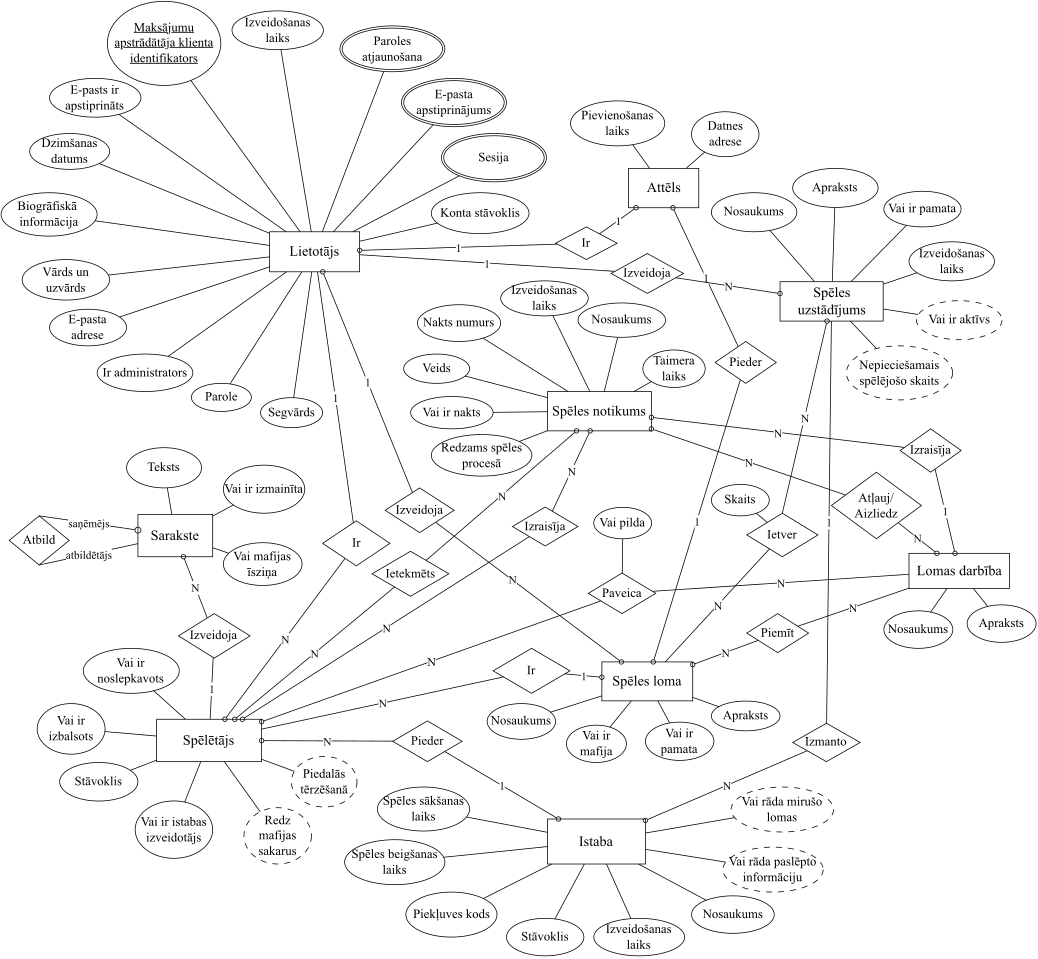
\includegraphics[width=\linewidth]{./src/img/KonceptualaisERModelis.png} % TODO: replace with correct picture
	\caption{Datu bāzes loģiskais ER modelis}
	\label{fig:logical-model}
\end{figure}

\subsection{Datu bāzes tabulu apraksts}
Datubāzes tabulu lauku, datu tipi, lauka atribūti - obligātums, noklusētās vērtības, primārā atslēga,
unikalitāte - ir aprakstītas atsevišķās tabulās (skat. x.1, x.2, … , x.n tab. % TODO: add all table references).
Visām tabulām, \texttt{VARCHAR} un \texttt{TEXT} laukiem tiek lietots UTF8 kodējums.

\begin{entityTable}{LomasDarbiba}{entity-role-action}
	\entityTableRow{nosaukums}{varchar(255)}{unique, not null}{Lomas darbības nosaukums}
	\entityTableRow{is\_nekavejoties}{bool}{default false, not null}{Vai lomas darbība ir tūlītēja}
\end{entityTable}

\begin{entityTable}{LomasTrukums}{entity-role-disadvantage}
	\entityTableRow{nosaukums}{varchar(255)}{unique, not null}{Lomas trūkuma nosaukums}
	\entityTableRow{apraksts}{text}{default '', not null}{Lomas trūkuma apraksts}
\end{entityTable}

\begin{entityTable}{Attels}{entity-image}
	\entityTableRow{datnes\_adrese}{varchar(255)}{unique, not null}{Saglabātā attēla adrese operētājsistēmā}
	\entityTableRow{pievienosanas\_laiks}{timestamp}{default current\_timestamp, not null}{Laiks, kad tika izveidots/saglabāts dotais attēls datubāzē}
\end{entityTable}

\begin{entityTable}{AbonementaCena}{entity-subscription-price}
	\entityTableRow{cena}{decimal(16,2)}{default 0, not null, check (cena >= 0)}{Abonementa cena, kuras garums var būt līdz 16 simboliem un tiek noapaļots līdz 2 cipariem aiz komata} % FIX: `cena` should be in lowercase
	\entityTableRow{pievienosanas\_laiks}{timestamp}{default current\_timestamp, not null}{Laiks, kad tika izveidots/saglabāts dotā cena datubāzē}
	\entityTableRow{aktivizesanas\_laiks}{timestamp}{not null, check (aktivizesanas\_laiks >= pievienosanas\_laiks)}{Laiks, no kura ši cena ir aktīva} % FIX: should be in lowercase
\end{entityTable}

\begin{entityTable}{ParolesAtjaunosana}{entity-password-recovery}
	\entityTableRow{markieris}{varchar(255)}{unique, not null}{Ģenerēts marķieris e-pasta lietotāja paroles atjaunošanai}
	\entityTableRow{deriguma\_termins}{timestamp}{not null}{Laiks, līdz kurams paroles atjaunošana ir iespējama}
\end{entityTable}

\begin{entityTable}{EpastaApstiprinajums}{entity-email-confirmation}
	\entityTableRow{markieris}{varchar(255)}{unique, not null}{Ģenerēts marķieris e-pasta lietotāja apstiprināšanai}
	\entityTableRow{deriguma\_termins}{timestamp}{not null}{Laiks, līdz kuram e-pasta apstiprināšana ir iespējama}
\end{entityTable}

\begin{entityTable}{SpelesLoma}{entity-game-role}
	\entityTableRow{nosaukums}{varchar(255)}{unique, not null}{Lomas nosaukums}
	\entityTableRow{apraksts}{text}{default '', not null}{Lomas apraksts}
	\entityTableRow{max\_speletaju\_ skaits}{int4}{default 1, not null, check (\lowercase{max\_speletaju\_ skaits} > 0)}{Maksimālais spēlētāju skaits spēlē ar doto lomu}
	\entityTableRow{ir\_pamata}{bool}{default false, not null}{Vai loma ir spēles pamatā vai lietotāju izveidots?}
	\entityTableRow{ir\_mafija}{bool}{default false, not null}{Vai loma ir mafija?}
	\entityTableRow{attels}{int8}{}{Lomas attēls, \texttt{FOREING KEY} uz \hyperref[tab:entity-image]{Attels} tabulas id kolonnu}
\end{entityTable}

\begin{entityTable}{KontaStavoklis}{entity-account-status}
	\entityTableRow{teksts}{varchar(255)}{unique, not null}{Konta stāvokļa apraksts}
\end{entityTable}

\begin{entityTable}{AbonementaStavoklis}{entity-subscription-status}
	\entityTableRow{teksts}{varchar(255)}{unique, not null}{Abonementa stāvokļa apraksts}
\end{entityTable}

\begin{entityTable}{IstabasStavoklis}{entity-room-status}
	\entityTableRow{teksts}{varchar(255)}{unique, not null}{Istabas stāvokļa apraksts}
\end{entityTable}

\begin{entityTable}{Lietotajs}{entity-user}
	\entityTableRow{segvards}{varchar(255)}{unique, not null}{Lietotājvārds}
	\entityTableRow{epasts}{varchar(255)}{unique, not null}{Lietotāja e-pasts}
	\entityTableRow{parole}{varchar(255)}{not null}{Šifrēta lietotāja parole}
	\entityTableRow{vards}{varchar(255)}{default '', not null}{Lietotāja vārds}
	\entityTableRow{uzvards}{varchar(255)}{default '', not null}{Lietotāja uzvārds}
	\entityTableRow{dzimsanas\_datums}{date}{}{Lietotāja dzimšanas datums}
	\entityTableRow{bio\_info}{text}{default ''}{Lietotāja apraksts par sevi}
	\entityTableRow{izveidosanas\_laiks}{timestamp}{not null, default current\_timestamp}{Laiks, kad tika izveidots/saglabāts dotais lietotājs datubāzē}
	\entityTableRow{attels}{int8}{}{Lietotāja profila attēls, \texttt{FOREING KEY} uz \hyperref[tab:entity-image]{Attels} tabulas id kolonnu}
	\entityTableRow{konta\_stavoklis}{int8}{}{Lietotāja konta stāvoklis, \texttt{FOREING KEY} uz \hyperref[tab:entity-account-status]{KontaStavoklis} tabulas id kolonnu}
	\entityTableRow{epasta\_apstiprinajums}{int8}{}{Lietotāja e-pasta apstiprinājums, \texttt{FOREING KEY} uz \hyperref[tab:entity-email-confirmation]{EpastaApstiprinajums} tabulas id kolonnu}
	\entityTableRow{paroles\_atjaunosana}{int8}{}{Lietotāja paroles atjaunošana, \texttt{FOREING KEY} uz \hyperref[tab:entity-password-recovery]{ParolesAtjaunojana} tabulas id kolonnu}
\end{entityTable}

\begin{entityTable}{SpelesKonfiguracija}{enity-game-setup}
	\entityTableRow{nosaukums}{varchar(255)}{unique, not null}{Konfigurācijas nosaukums}
	\entityTableRow{apraksts}{text}{default '', not null}{Konfigurācijas apraksts}
	\entityTableRow{ir\_pamata}{bool}{default false, not null}{Vai spēles konfigurācijas ir spēles pamatā vai lietotāju izveidots}
	\entityTableRow{izveidosanas\_laiks}{timestamp}{not null, default current\_timestamp}{Laiks, kad dotais uzstādījums tika izveidots/saglabāts datubāzē}
	\entityTableRow{autors}{int8}{not null}{Konfigurācijas autors, \texttt{FOREING KEY} uz \hyperref[tab:entity-user]{Lietotajs} tabulas id kolonnu}
\end{entityTable}

\begin{entityTable}{Istaba}{entity-room}
	\entityTableRow{nosaukums}{varchar(255)}{unique, not null}{Istabas Nosaukums}
	\entityTableRow{speles\_saksanas\_laiks}{timestamp}{}{Laiks, kad spēle sākas}
	\entityTableRow{speles\_beigsanas\_laiks}{timestamp}{}{Laiks, kad spēle beidzas}
	\entityTableRow{stavoklis}{int8}{not null}{Pašreizējais spēles stāvoklis, \texttt{FOREING KEY} uz \hyperref[tab:entity-room-status]{IstabasStavoklis} tabulas id kolonnu}
	\entityTableRow{piekluves\_kods}{char(6)}{unique}{Unikāls istabas piekļuves kods, 6 lielie burtcipari}
	\entityTableRow{vai\_rada\_miruso\_lomu}{bool}{default false, not null}{Vai pēc spēlētāja nāves var atklāt viņa lomu?}
	\entityTableRow{izveidosanas\_laiks}{timestamp}{default current\_timestamp, not null}{Laiks, kad dotā spēles istaba tika izveidota/saglabāta datubāzē}
	\entityTableRow{speles\_konfiguracija}{int8}{not null}{Spēles uzstādījumi, kurus izmanto dotā istaba, \texttt{FOREING KEY} uz \hyperref[tab:entity-game-setup]{SpelesKonfiguracija} tabulas id kolonnu}
\end{entityTable}

\begin{entityTable}{SpelesNotikums}{entity-game-event}
	\entityTableRow{nosaukums}{varchar(255)}{unique, not null}{Notikuma nosaukums}
	\entityTableRow{nakts\_pk}{int2}{default 0, not null, check (nakts\_pk >= 0)}{Spēles nakts pēc kārtas} % FIX: 
	\entityTableRow{ir\_redzams}{bool}{default false, not null}{Vai notikums ir redzams spēlētājiem procesa laikā?}
	\entityTableRow{izveidosanas\_laiks}{timestamp}{not null, default current\_timestamp}{Laiks, kad dotais spēles notikums tika izveidots/saglabāts datubāzē}
\end{entityTable}



% \input{./src/test.tex}

\end{document}
